% Created by tikzDevice version 0.12.6 on 2026-08-03 03:40:41
% !TEX encoding = UTF-8 Unicode
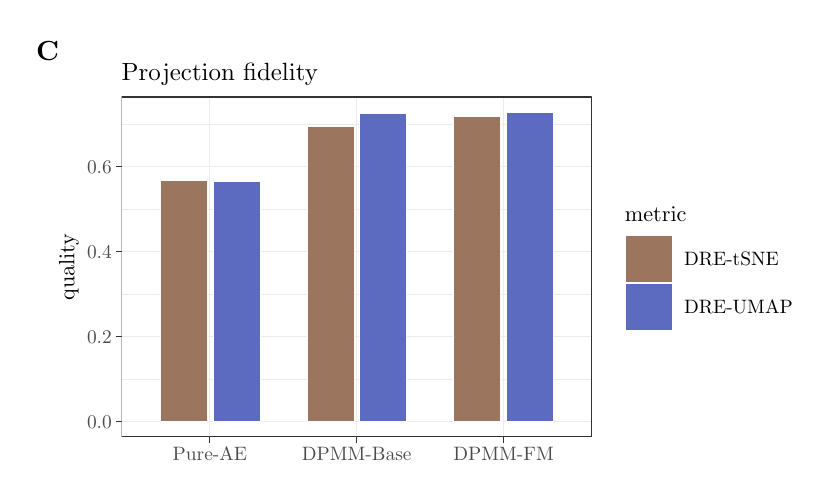
\begin{tikzpicture}[x=1pt,y=1pt]
\definecolor{fillColor}{RGB}{255,255,255}
\path[use as bounding box,fill=fillColor,fill opacity=0.00] (0,0) rectangle (283.45,161.83);
\begin{scope}
\path[clip] (  1.05,  1.74) rectangle (282.41,160.09);
\definecolor{drawColor}{RGB}{255,255,255}
\definecolor{fillColor}{RGB}{255,255,255}

\path[draw=drawColor,line width= 0.4pt,line join=round,line cap=round,fill=fillColor] (  1.05,  1.74) rectangle (282.41,160.09);
\end{scope}
\begin{scope}
\path[clip] ( 33.99, 13.93) rectangle (203.83,136.79);
\definecolor{fillColor}{RGB}{255,255,255}

\path[fill=fillColor] ( 33.99, 13.93) rectangle (203.83,136.79);
\definecolor{drawColor}{gray}{0.92}

\path[draw=drawColor,line width= 0.2pt,line join=round] ( 33.99, 34.86) --
	(203.83, 34.86);

\path[draw=drawColor,line width= 0.2pt,line join=round] ( 33.99, 65.53) --
	(203.83, 65.53);

\path[draw=drawColor,line width= 0.2pt,line join=round] ( 33.99, 96.21) --
	(203.83, 96.21);

\path[draw=drawColor,line width= 0.2pt,line join=round] ( 33.99,126.89) --
	(203.83,126.89);

\path[draw=drawColor,line width= 0.4pt,line join=round] ( 33.99, 19.52) --
	(203.83, 19.52);

\path[draw=drawColor,line width= 0.4pt,line join=round] ( 33.99, 50.20) --
	(203.83, 50.20);

\path[draw=drawColor,line width= 0.4pt,line join=round] ( 33.99, 80.87) --
	(203.83, 80.87);

\path[draw=drawColor,line width= 0.4pt,line join=round] ( 33.99,111.55) --
	(203.83,111.55);

\path[draw=drawColor,line width= 0.4pt,line join=round] ( 65.84, 13.93) --
	( 65.84,136.79);

\path[draw=drawColor,line width= 0.4pt,line join=round] (118.91, 13.93) --
	(118.91,136.79);

\path[draw=drawColor,line width= 0.4pt,line join=round] (171.98, 13.93) --
	(171.98,136.79);
\definecolor{drawColor}{RGB}{255,255,255}
\definecolor{fillColor}{RGB}{92,107,192}

\path[draw=drawColor,line width= 0.2pt,fill=fillColor] (119.97, 19.52) rectangle (136.95,130.86);

\path[draw=drawColor,line width= 0.2pt,fill=fillColor] (173.04, 19.52) rectangle (190.03,131.21);

\path[draw=drawColor,line width= 0.2pt,fill=fillColor] ( 66.90, 19.52) rectangle ( 83.88,106.21);
\definecolor{fillColor}{RGB}{156,117,95}

\path[draw=drawColor,line width= 0.2pt,fill=fillColor] (100.86, 19.52) rectangle (117.85,126.27);

\path[draw=drawColor,line width= 0.2pt,fill=fillColor] (153.94, 19.52) rectangle (170.92,129.67);

\path[draw=drawColor,line width= 0.2pt,fill=fillColor] ( 47.79, 19.52) rectangle ( 64.77,106.75);
\definecolor{drawColor}{gray}{0.20}

\path[draw=drawColor,line width= 0.4pt,line join=round,line cap=round] ( 33.99, 13.93) rectangle (203.83,136.79);
\end{scope}
\begin{scope}
\path[clip] (  0.00,  0.00) rectangle (283.45,161.83);
\definecolor{drawColor}{gray}{0.30}

\node[text=drawColor,anchor=base east,inner sep=0pt, outer sep=0pt, scale=  0.70] at ( 30.39, 17.11) {0.0};

\node[text=drawColor,anchor=base east,inner sep=0pt, outer sep=0pt, scale=  0.70] at ( 30.39, 47.78) {0.2};

\node[text=drawColor,anchor=base east,inner sep=0pt, outer sep=0pt, scale=  0.70] at ( 30.39, 78.46) {0.4};

\node[text=drawColor,anchor=base east,inner sep=0pt, outer sep=0pt, scale=  0.70] at ( 30.39,109.14) {0.6};
\end{scope}
\begin{scope}
\path[clip] (  0.00,  0.00) rectangle (283.45,161.83);
\definecolor{drawColor}{gray}{0.20}

\path[draw=drawColor,line width= 0.4pt,line join=round] ( 31.99, 19.52) --
	( 33.99, 19.52);

\path[draw=drawColor,line width= 0.4pt,line join=round] ( 31.99, 50.20) --
	( 33.99, 50.20);

\path[draw=drawColor,line width= 0.4pt,line join=round] ( 31.99, 80.87) --
	( 33.99, 80.87);

\path[draw=drawColor,line width= 0.4pt,line join=round] ( 31.99,111.55) --
	( 33.99,111.55);
\end{scope}
\begin{scope}
\path[clip] (  0.00,  0.00) rectangle (283.45,161.83);
\definecolor{drawColor}{gray}{0.20}

\path[draw=drawColor,line width= 0.4pt,line join=round] ( 65.84, 11.93) --
	( 65.84, 13.93);

\path[draw=drawColor,line width= 0.4pt,line join=round] (118.91, 11.93) --
	(118.91, 13.93);

\path[draw=drawColor,line width= 0.4pt,line join=round] (171.98, 11.93) --
	(171.98, 13.93);
\end{scope}
\begin{scope}
\path[clip] (  0.00,  0.00) rectangle (283.45,161.83);
\definecolor{drawColor}{gray}{0.30}

\node[text=drawColor,anchor=base,inner sep=0pt, outer sep=0pt, scale=  0.70] at ( 65.84,  5.51) {Pure-AE};

\node[text=drawColor,anchor=base,inner sep=0pt, outer sep=0pt, scale=  0.70] at (118.91,  5.51) {DPMM-Base};

\node[text=drawColor,anchor=base,inner sep=0pt, outer sep=0pt, scale=  0.70] at (171.98,  5.51) {DPMM-FM};
\end{scope}
\begin{scope}
\path[clip] (  0.00,  0.00) rectangle (283.45,161.83);
\definecolor{drawColor}{RGB}{0,0,0}

\node[text=drawColor,rotate= 90.00,anchor=base,inner sep=0pt, outer sep=0pt, scale=  0.80] at ( 16.86, 75.36) {quality};
\end{scope}
\begin{scope}
\path[clip] (  0.00,  0.00) rectangle (283.45,161.83);
\definecolor{fillColor}{RGB}{255,255,255}

\path[fill=fillColor] (211.83, 48.25) rectangle (280.41,102.47);
\end{scope}
\begin{scope}
\path[clip] (  0.00,  0.00) rectangle (283.45,161.83);
\definecolor{drawColor}{RGB}{0,0,0}

\node[text=drawColor,anchor=base west,inner sep=0pt, outer sep=0pt, scale=  0.80] at (215.83, 91.95) {metric};
\end{scope}
\begin{scope}
\path[clip] (  0.00,  0.00) rectangle (283.45,161.83);
\definecolor{fillColor}{RGB}{255,255,255}

\path[fill=fillColor] (215.83, 69.60) rectangle (233.17, 86.94);
\definecolor{drawColor}{RGB}{255,255,255}
\definecolor{fillColor}{RGB}{156,117,95}

\path[draw=drawColor,line width= 0.2pt,fill=fillColor] (216.11, 69.88) rectangle (232.89, 86.66);
\end{scope}
\begin{scope}
\path[clip] (  0.00,  0.00) rectangle (283.45,161.83);
\definecolor{fillColor}{RGB}{255,255,255}

\path[fill=fillColor] (215.83, 52.25) rectangle (233.17, 69.60);
\definecolor{drawColor}{RGB}{255,255,255}
\definecolor{fillColor}{RGB}{92,107,192}

\path[draw=drawColor,line width= 0.2pt,fill=fillColor] (216.11, 52.54) rectangle (232.89, 69.31);
\end{scope}
\begin{scope}
\path[clip] (  0.00,  0.00) rectangle (283.45,161.83);
\definecolor{drawColor}{RGB}{0,0,0}

\node[text=drawColor,anchor=base west,inner sep=0pt, outer sep=0pt, scale=  0.70] at (237.17, 75.86) {DRE-tSNE};
\end{scope}
\begin{scope}
\path[clip] (  0.00,  0.00) rectangle (283.45,161.83);
\definecolor{drawColor}{RGB}{0,0,0}

\node[text=drawColor,anchor=base west,inner sep=0pt, outer sep=0pt, scale=  0.70] at (237.17, 58.51) {DRE-UMAP};
\end{scope}
\begin{scope}
\path[clip] (  0.00,  0.00) rectangle (283.45,161.83);
\definecolor{drawColor}{RGB}{0,0,0}

\node[text=drawColor,anchor=base west,inner sep=0pt, outer sep=0pt, scale=  0.90] at ( 33.99,142.78) {Projection fidelity};
\end{scope}
\begin{scope}
\path[clip] (  0.00,  0.00) rectangle (283.45,161.83);
\definecolor{drawColor}{RGB}{0,0,0}

\node[text=drawColor,anchor=base,inner sep=0pt, outer sep=0pt, scale=  1.00] at (  7.20,150.08) {\bfseries C};
\end{scope}
\end{tikzpicture}
